\documentclass[10pt,compress,mathserif]{beamer}
\usetheme{Copenhagen}
% Few theme names Berkeley Copenhagen Dresden


\usepackage{amsmath,minibox,amssymb,amsfonts,amsthm,graphicx,color,multirow,array,tikz,hyperref}
\usetikzlibrary{arrows,snakes,backgrounds,patterns,matrix,shapes,fit,calc,shadows, positioning}

\setbeamertemplate{navigation symbols}{} % This is just to get rid of the extra fazool symbols
\setbeamerfont{caption}{size=\footnotesize}

\title[]{Control Systems Project}
\author[]{Mian Inshaullah \\18PWCSE1721 \\ Section C, DCSE \\ UET Peshawar.}
\rightskip=0pt plus 0pt
\boldmath

\begin{document}
\begin{frame}    \titlepage \end{frame}

% First slide
\section{Introduction}
\begin{frame}{Introduction to Project}
\noindent A hard disk is a data storage device. It uses magnetic storage system with electronic hardware to access the data. The electronic circuit consists of a dc motor. A dc motor has the following state space\\ \vskip10pt
\begin{equation}
\begin{bmatrix} \dot{\theta}\\  \dot{\Theta} \\ \dot{i}\end{bmatrix}
= \begin{bmatrix}
0 & 1 & 0 \\
0 & \frac{-b}{J} & \frac{k}{J} \\
0 & \frac{k}{L} & \frac{-R}{L}  \end{bmatrix}
\begin{bmatrix} \theta\\  \Theta \\ i \end{bmatrix} +
\begin{bmatrix}
0 \\
0 \\
\frac{1}{L}  \end{bmatrix}
 u 
\end{equation}\vskip10pt

\begin{equation}
y(t)=\begin{bmatrix}
1 & 0 & 0
\end{bmatrix}
\begin{bmatrix} \theta \\  \Theta \\ i \end{bmatrix}
\end{equation}
\end{frame}

\begin{frame}{Introduction to Project}
a. Use J = 3.2, b = 3.5, k = 0.0274, R = 4, and L = 2.75; Check the stability of the system using all methods that you know \\ \vskip10pt
b. Simulate the unstable system and show that its response is unstable \\ \vskip10pt
c. Compute the controllability matrix for the system. If the system is controllable, place the controller eigenvalues at (-14, -33, -33) and observer eigenvalues at a location which is faster than the controller eigenvalues.\\ \vskip10pt
d. Simulate the stable system and show its response \\ 
\vskip10pt
e. Design a PID Controller and compare it with response obtained from part d\\ \vskip10pt
f. Compute the steady state errors before and after designing controller\\ \vskip10pt
g. Design a tracking controller for step tracking of amplitude 5u(t) and ramp tracking of 5tu(t)\\ 
\end{frame}



% Second Slide
\section{Solution}
\begin{frame}{State-space Representation of the System}
The state-space representation of the system can be written as follows:
\begin{equation}
\begin{bmatrix} \dot{\theta}\\  \dot{\Theta} \\ \dot{i}\end{bmatrix}
= \begin{bmatrix}
0 & 1 & 0 \\
0 & -1.0938 & 0.0086 \\
0 & 0.01 & -1.4545  \end{bmatrix}
\begin{bmatrix} \theta\\  \Theta \\ i \end{bmatrix} +
\begin{bmatrix}
0 \\
0 \\
0.3636  \end{bmatrix}
 u 
\end{equation}\vskip10pt


\begin{equation}
y(t)=\begin{bmatrix}
1 & 0 & 0
\end{bmatrix}
\begin{bmatrix} \theta \\  \Theta \\ i \end{bmatrix}
\end{equation}

\end{frame}


\section{Stability Analysis}
\begin{frame}{Stability Analysis of the System}
\textbf{The Transfer Function of the System is as follows:} 
\begin{equation}
\frac{0.003114}{s^3 + 2.548s^2 + 1.591s}
\end{equation}

\textbf{The Eigenvalues of the system are:}

\begin{equation} \lambda_1 = 0,   \lambda_2 = -1.4545,  \lambda_3 = -1.0935 \end{equation}
\vskip10pt
The eigenvalues of the system were computed using \textit{eig(A)} matlab function
\vskip10pt

\textbf{The poles of the system are: }
\begin{equation} p_1 = 0 ,  p_2 = -1.0935 ,  p_3 =-1.4545  \end{equation}
The poles of the system were computed using the \textit{roots(denum)} matlab function. 

\vskip10pt
Considering one of the eigenvalues and one of the poles is equal to zero, it indicates the system is marginally stable. 
\end{frame}

\begin{frame}{Stability Analysis of the System}
Routh-Hurwitz table is shown below
\begin{table}[h] \begin{center}
\begin{tabular}{|l|c|l|} \hline
$s^3$  & 1 & 1.591\\ \hline
$s^2$ & 2.548 & 0 \\ \hline
$s^1$  & $-\frac{1}{2.548}\times\begin{vmatrix} 1 & 1.591\\ 2.548 & 0 \end{vmatrix}=1.5910$ & 0 \\ \hline
$s^0$  & $-\frac{1}{-1.5910}\times\begin{vmatrix} 1.591 & 0\\ 1.591 & 0 \end{vmatrix}=0$ & 0 \\ \hline
\end{tabular} \end{center}
\end{table}

Sign has not changed in the first column; therefore, the system is stable. 


\end{frame}


\begin{frame}{Stability Analysis of the System}
The step response of the system is as below: System is unbounded, which means it's marginally stable. 
\vskip10pt
\begin{figure}[h!]
\centering
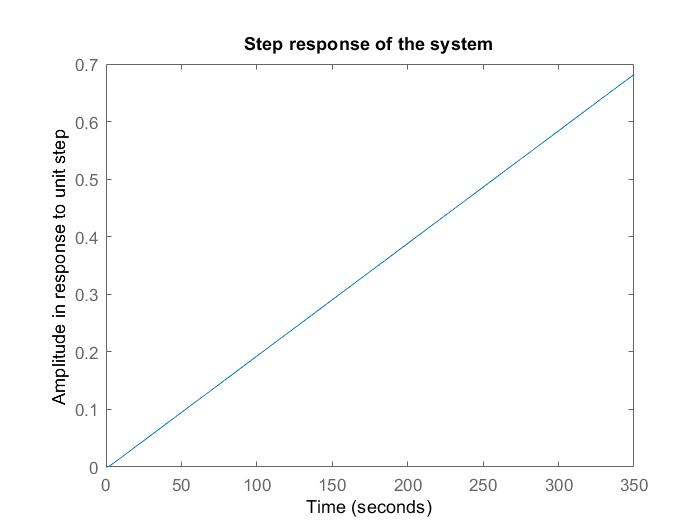
\includegraphics[scale=0.25]{Step_response.jpg}
\caption{Plot of step response.}
\end{figure}


\end{frame}


\begin{frame}{Stability Analysis of the System}
The Root locus plot of the system is as below: At gain k = 0, system is marginally stable
\begin{figure}[h!]
\centering
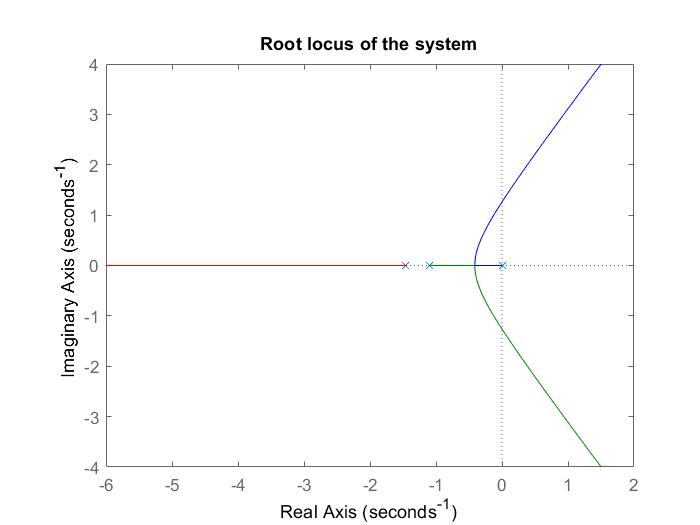
\includegraphics[scale=0.3]{root_locus.jpg}
\caption{Plot of root locus.}
\end{figure}
\end{frame}



\section{Controllability}
\begin{frame}{Controllability Analysis}


\vskip10pt
\begin{equation} P = ctrb(A, B) \end{equation}\vskip10pt
\begin{equation}
\begin{bmatrix}
\
0 & 0 & 0.0031 \\
0 & 0.0031 & -0.0079 \\
0.3636 & -0.5289 & 0.7694  \end{bmatrix}
\end{equation}
\vskip10pt
\begin{equation}
Ctrb rank = rank(P)
\end{equation}

\begin{equation}
 Ctrbrank = 3
\end{equation}
\begin{itemize}
\item As rank of Matrix P is same as matrix A, we conclude that the system passes controllability test. 
\item Since the system is controllable, we place controller eigen values at (-14, -33, -33)
\end{itemize}
 
\vskip10pt
\end{frame}


\section{Observability}
\begin{frame}{Observability Analysis}
\begin{equation} Q = obsv(A, C) \end{equation}
\begin{equation}
\begin{bmatrix}
\
1 & 0 & 0 \\
0 & 1 & 0\\
0 & -1.0938 & 0.0086  \end{bmatrix}
\end{equation}

\begin{equation}
Obsv rank = obsv(Q)
\end{equation}

\begin{equation}
 Obsvrank = 3
\end{equation}
\begin{itemize}
\item As rank of Matrix Q is same as matrix A, we conclude that the system passes observability test. 
\item Since the system is controllable, we place controller eigenvalues at (-15, -34, -34) \end{itemize}
\end{frame}

\section{Controller Design in Simulink}
\begin{frame}{Controller Design in Simulink}
\begin{equation}
L = \begin{bmatrix}
80.4517 \\
1.9694 * 10^3 \\
1.6756 * 10^6 \end{bmatrix}
\end{equation}
\begin{equation}
K = 
\begin{bmatrix}
4.8965*10^6 & 6.1879*10^5 & 212.9922 
\end{bmatrix}
\end{equation}

\begin{equation}
B(obv) = 
\begin{bmatrix}
B & L \\
\end{bmatrix}
\end{equation}
\begin{equation}
B(obv) = 
\begin{bmatrix}
0 & 80.4517\\
0 & 1.9694 * 10^3\\
0.3636 & 1.6756* 10^6\\\end{bmatrix}
\end{equation}

\end{frame}


\section{Schematics}
\begin{frame}{Schematics - Marginally Stable System}
\vskip10pt
\begin{figure}[h!]
\centering
\includegraphics[scale=0.6]{marginallystablesystem.png}
\caption{Schematic of Marginally Stable System.}
\end{figure}




\end{frame}


\begin{frame}{Step Response}

(Simulink) The step response of the system is as below: System is unbounded, which means it's marginally stable. 
\vskip10pt
\begin{figure}[h!]
\centering
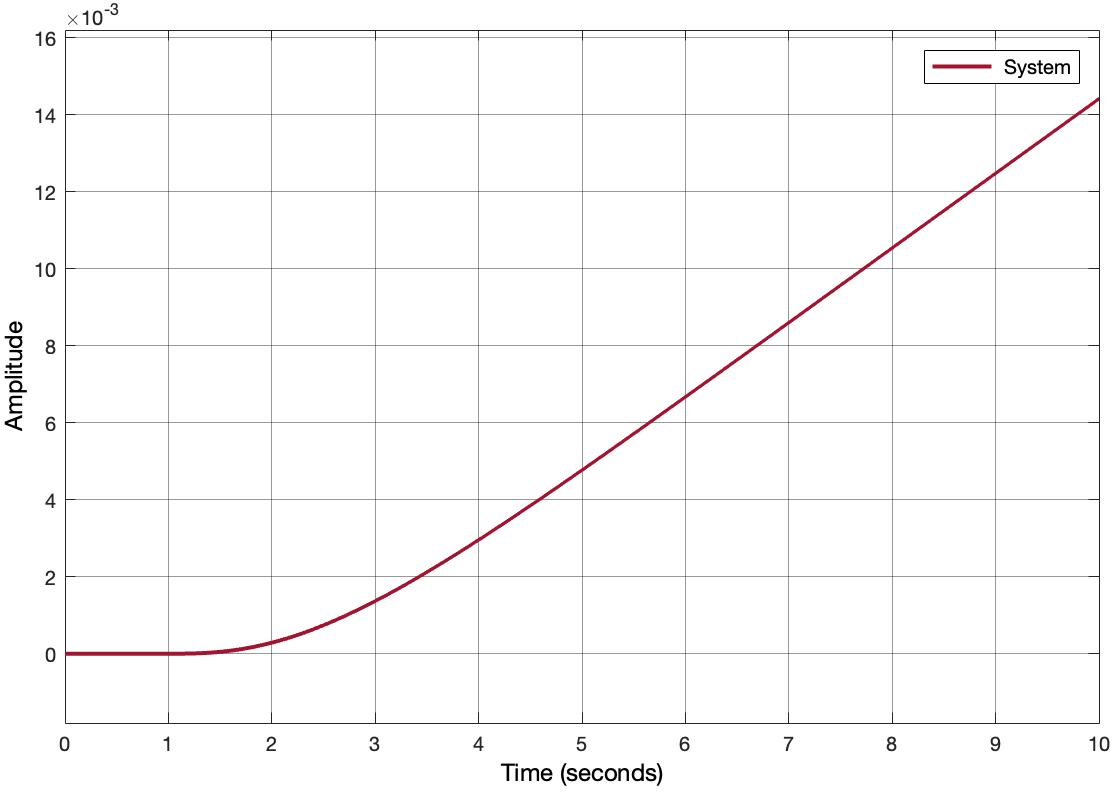
\includegraphics[scale=0.15]{UnstableSystem_response.jpg}
\caption{Plot of step response in simulink.}
\end{figure}

\end{frame}


\begin{frame}{Schematics - Marginally Stable System with Controller}
Schematic of Marginally Stable System after using observer-based feedback controller
\vskip10pt
\begin{figure}[h!]
\centering
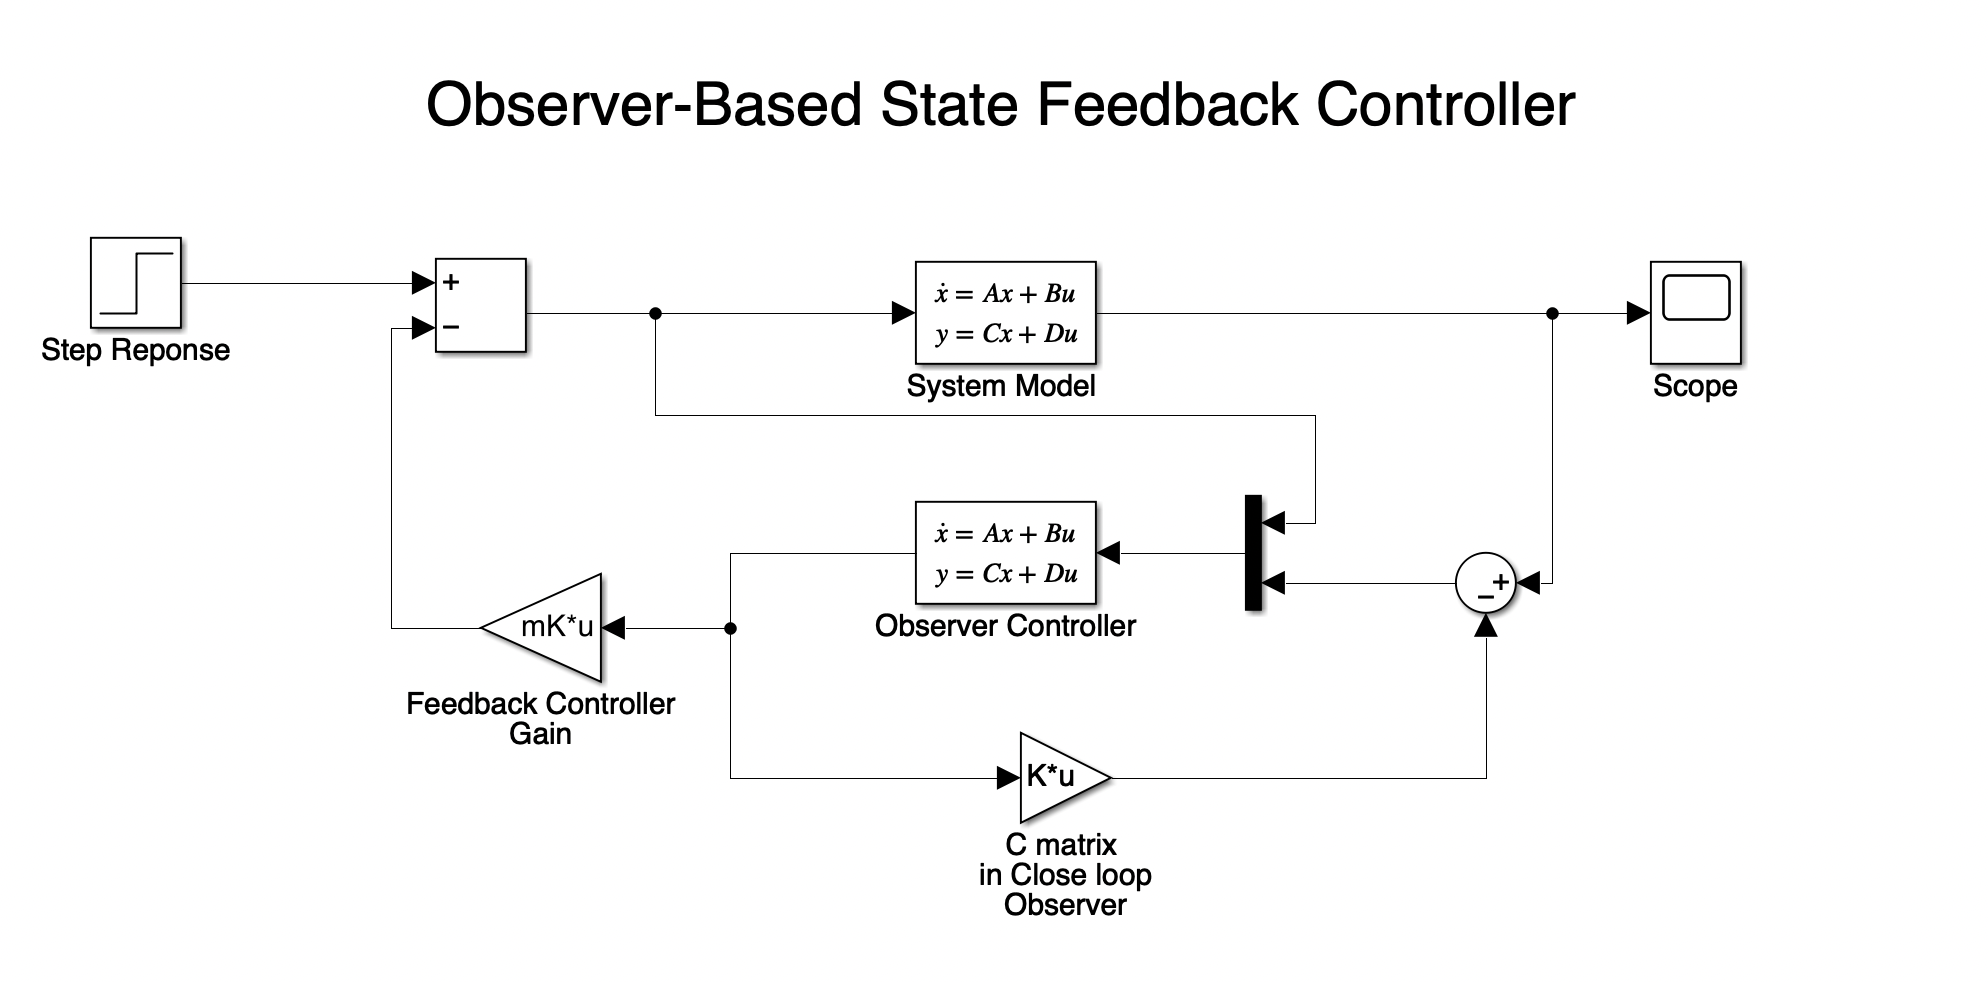
\includegraphics[scale=0.3]{ObserverbasedSFC.jpeg}
\caption{Schematic of Observer based State Feedback Controller.}
\end{figure}

\end{frame}

\end{frame}

\begin{frame}{Step Response}
Step Response of Marginally Stable System after using observer-based feedback controller

\vskip10pt
\begin{figure}[h!]
\centering
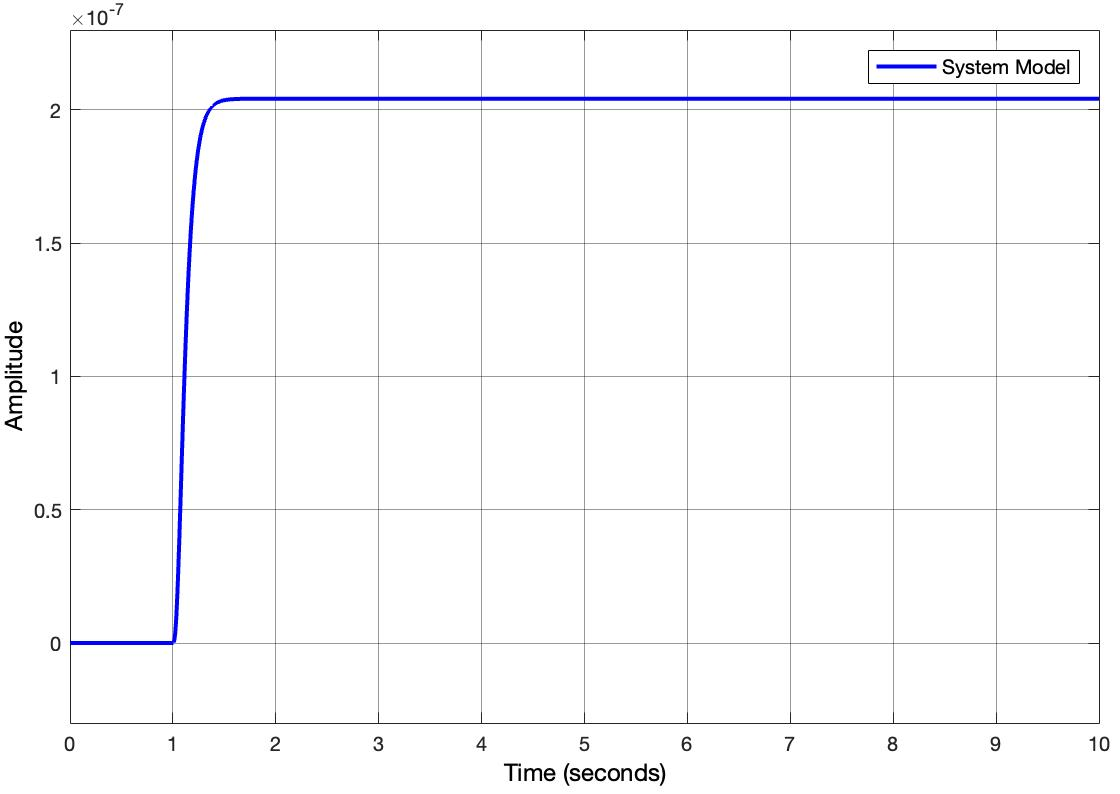
\includegraphics[scale=0.2]{ObserverbasedSFC_response.jpg}
\caption{Plot of Step Response of Observer based State Feedback Controller.}
\end{figure}

\end{frame}

\begin{frame}{Step Response Details}
\begin{itemize}
\item Rise Time = 0.196 seconds
\item Settling Time = 0.3580 seconds
\item Overshoot = 0
\item Undershoot = 0
\item Final Value = \begin{equation}
\frac{2.0417}{10^7}
\end{equation}
\end{itemize}
\end{frame}

\begin{frame}{Schematics - PID Controller with Controlled System}
Schematic of PID Controller with Controlled System

\vskip10pt
\begin{figure}[h!]
\centering
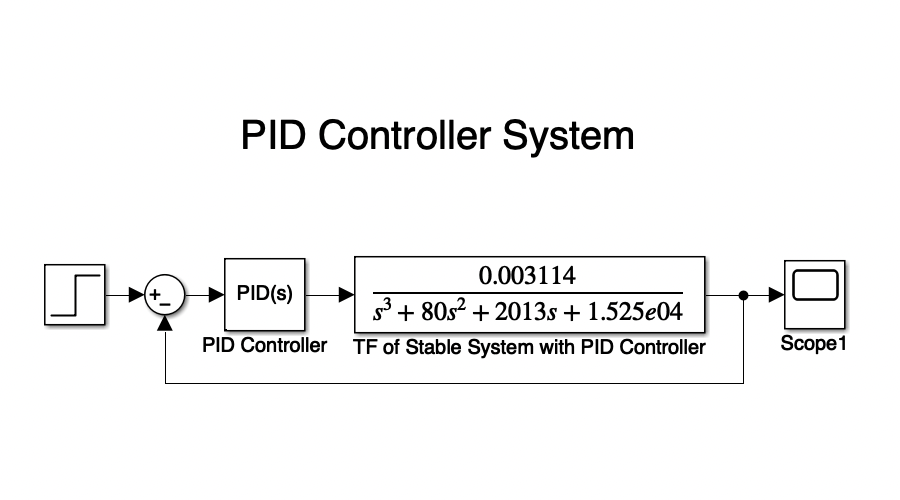
\includegraphics[scale=0.6]{PID_Model.png}
\caption{Schematic of PID Controller.}
\end{figure}

\end{frame}

\begin{frame}{Step Response}
Step Response of PID Controller with Controlled System
\vskip10pt
\begin{figure}[h!]
\centering
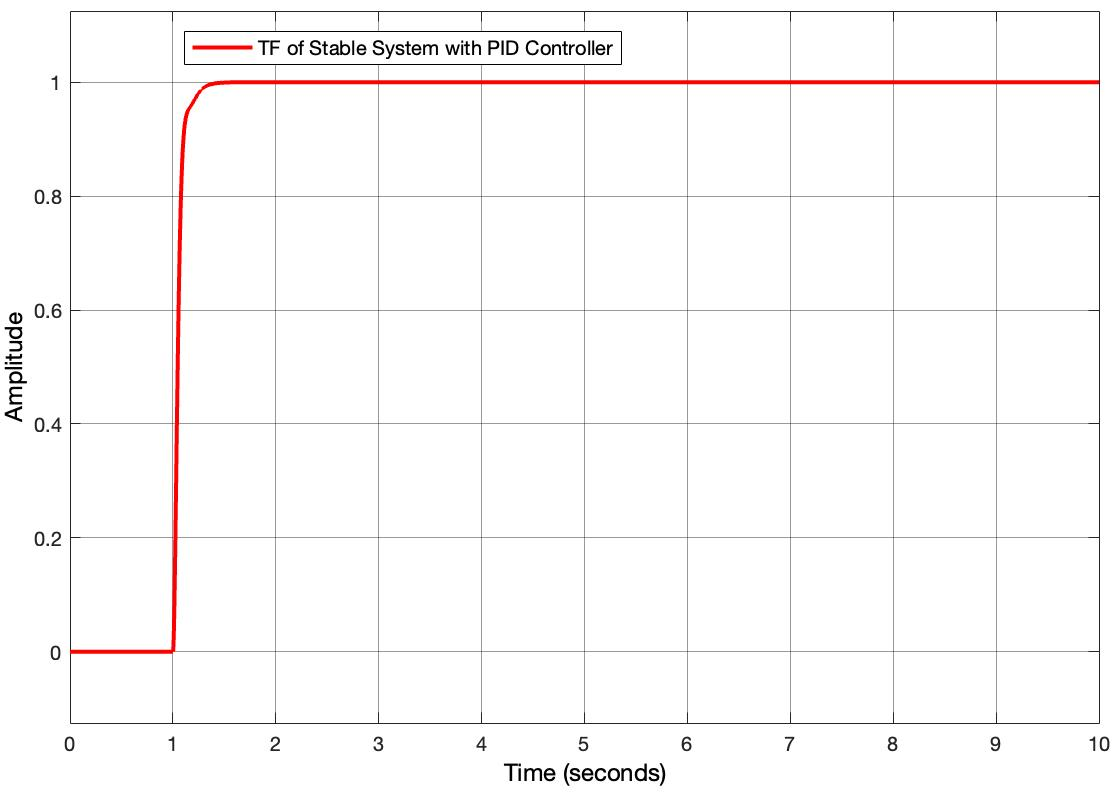
\includegraphics[scale=0.2]{pid_response.jpg}
\caption{Plot of Step Response of PID Controller.}
\end{figure}


\end{frame}

\begin{frame}{Step Response Details}
\begin{itemize}
\item Rise Time = 0.0844 seconds
\item Settling Time = 0.2257 seconds
\item Overshoot = 0
\item Undershoot = 0
\item Final Value = 1
\end{itemize}


\end{frame}

\begin{frame}{Comparison of  PID Controller with Controlled System}
Comparison of Step Responses from PID Controller and Controlled System

\vskip10pt
\begin{figure}[h!]
\centering
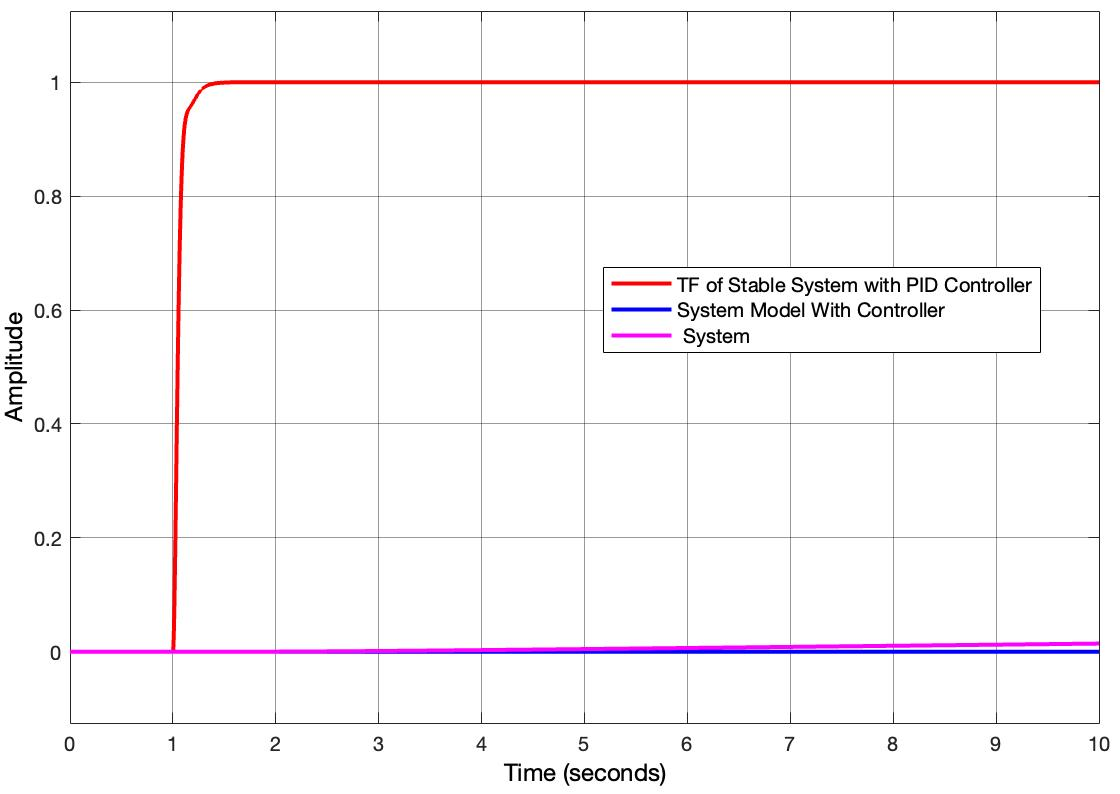
\includegraphics[scale=0.2]{Comparison.jpg}
\caption{Comparison of Step Responses of Observer based State Feedback Controller, PID Controller, and Marginally Stable System.}
\end{figure}
\end{frame}

\section{Steady State Errors}
\begin{frame}{Steady State Error}
\begin{itemize}
\item Steady State Error before the controller:
\begin{itemize}
\item Infinity or Undefined because system is unbounded. 
\end{itemize}

\item Steady State Error after Observer-based Feedback Controller
\begin{itemize}
\item  \begin{equation}
1 - \frac{2.0417}{10^7}\approx 1
\end{equation}
\end{itemize}

\item Steady State Error after PID Controller
\begin{itemize}
\item \begin{equation}
1 - 1 = 0 
\end{equation}
\end{itemize}
\end{itemize}
\begin{itemize}
\item Steady State Error for Ramp Input after Controller
\begin{itemize}
\item Infinity because system is Type 0
\end{itemize}
\item Steady State Error for Parabolic Input after Controller
\begin{itemize}
\item Infinity because system is Type 0
\end{itemize}
\end{itemize}

\end{frame}


\section{Designing a Tracking Controller}
\begin{frame}{Tracking Controller}
\begin{figure}[h!]
\centering
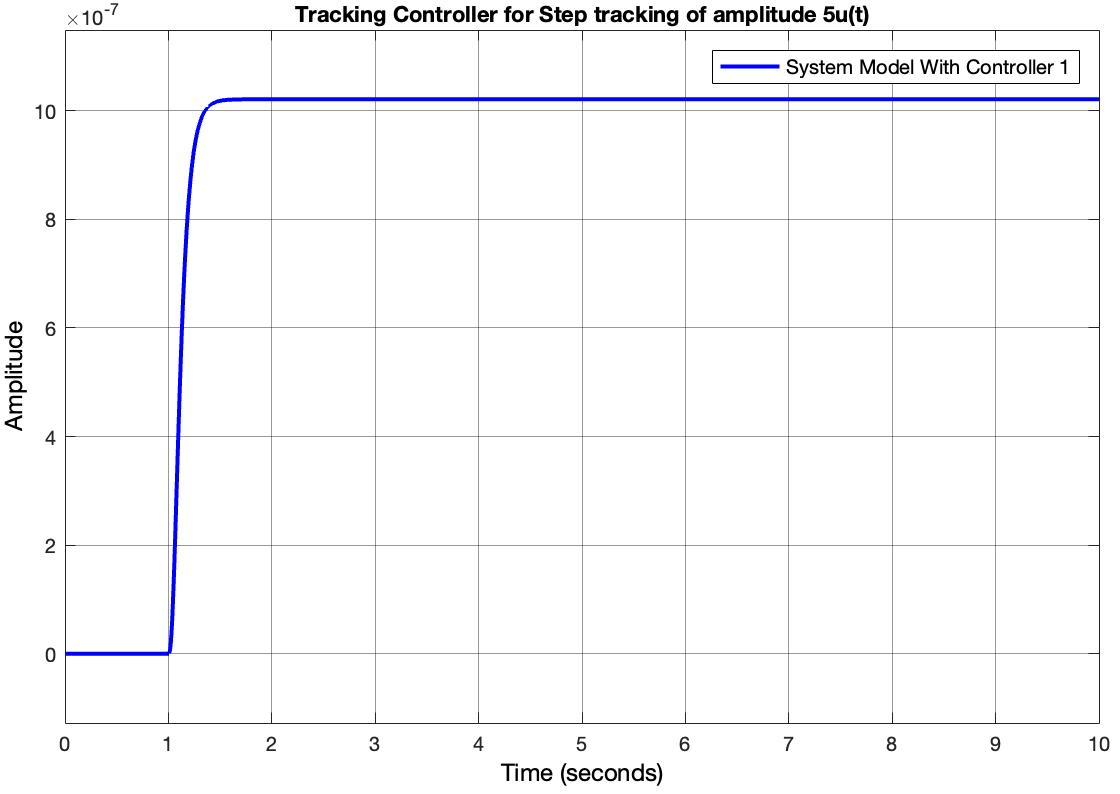
\includegraphics[scale=0.2]{Steptracking.jpg}
\caption{Plot of Step Tracking of amplitude 5u(t).}
\end{figure}
\end{frame}

\end{frame}

\begin{frame}{Tracking Controller}
\begin{figure}[h!]
\centering
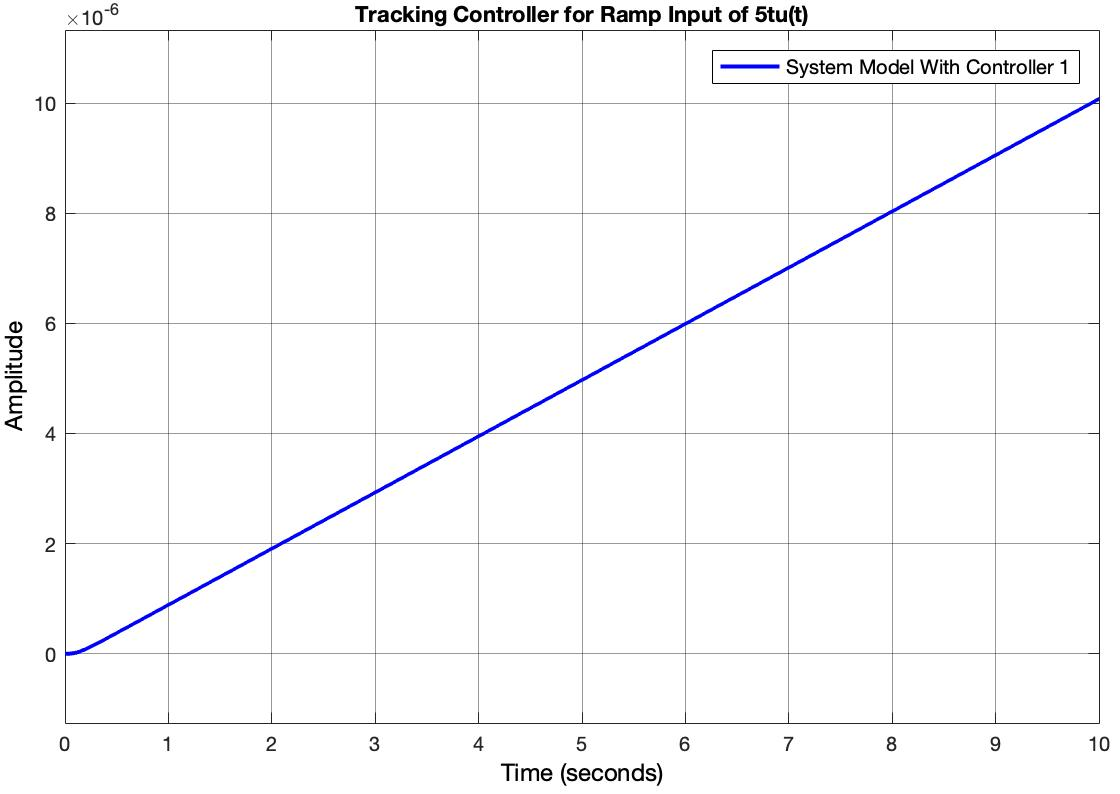
\includegraphics[scale=0.2]{TrackingControllerResponse.jpg}
\caption{Plot of Ramp Tracking of amplitude 5tu(t).}
\end{figure}
\end{frame}

\end{document} 